\chapterold{\RU{Файл сохранения состояния в игре Millenium}\EN{Millenium game save file}}
\label{Millenium_DOS_game}
\myindex{MS-DOS}

\RU{Игра}\EN{The} \q{Millenium Return to Earth} \RU{под DOS довольно древняя (1991), позволяющая
добывать ресурсы, строить корабли, снаряжать их на другие планеты,\etc{}.}
\EN{is an ancient DOS game (1991), that allows you to mine resources, build ships,
equip them on other planets, and so on}\footnote{\RU{Её можно скачать бесплатно}\EN{It can be downloaded for free}
\href{http://go.yurichev.com/17316}{\RU{здесь}\EN{here}}}.

\RU{Как и многие другие игры, она позволяет сохранять состояние игры в файл.}
\EN{Like many other games, it allows you to save all game state into a file.}

\RU{Посмотрим, сможем ли мы найти что-нибудь в нем}\EN{Let's see if we can find something in it}.

\clearpage
\RU{В игре есть шахта}\EN{So there is a mine in the game}.
\RU{Шахты на некоторых планетах работают быстрее, на некоторых других --- медленнее}\EN{Mines at some planets 
work faster, or slower on others}. 
\RU{Набор ресурсов также разный}\EN{The set of resources is also different}.

\RU{Здесь видно, какие ресурсы добыты в этот момент}\EN{Here we can see what resources are mined at the time}: 

\begin{figure}[H]
\centering
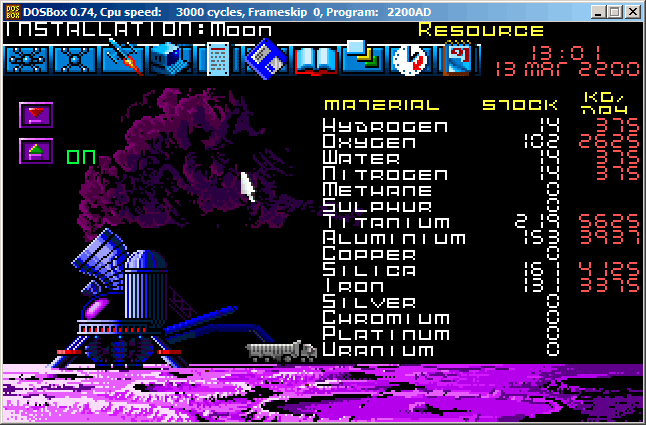
\includegraphics[scale=\FigScale]{ff/millenium/1.png}
\caption{\RU{Шахта: первое состояние}\EN{Mine: state 1}}
\label{fig:mill_1}
\end{figure}

\RU{Сохраним состояние игры}\EN{Let's save a game state}.
\RU{Это файл размером}\EN{This is a file of size} 9538 \RU{байт}\EN{bytes}.

\RU{Подождем несколько \q{дней} здесь в игре и теперь в шахте добыто больше ресурсов}%
\EN{Let's wait some \q{days} here in the game, and now we've got more resources from the mine}:

\begin{figure}[H]
\centering
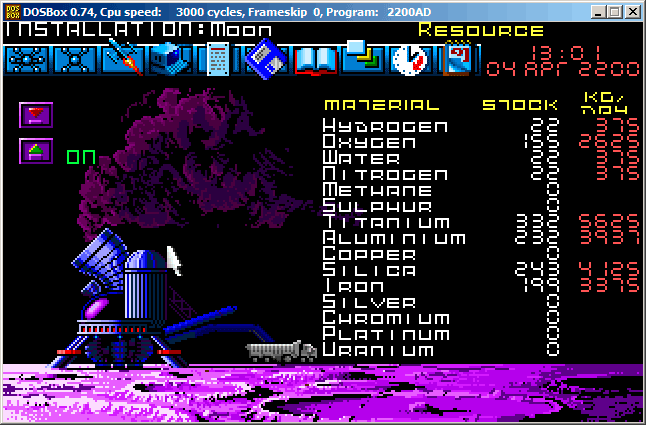
\includegraphics[scale=\FigScale]{ff/millenium/2.png}
\caption{\RU{Шахта: второе состояние}\EN{Mine: state 2}}
\label{fig:mill_2}
\end{figure}

\RU{Снова сохраним состояние игры}\EN{Let's sav game state again}.

\RU{Теперь просто попробуем сравнить оба файла побайтово используя простую утилиту FC под DOS/Windows:}
\EN{Now let's try to just do binary comparison of the save files using the simple DOS/Windows FC utility:}

\lstinputlisting{ff/millenium/fc_result.txt}

\RU{Вывод здесь неполный, там было больше отличий, но мы обрежем результат до самого интересного.}%
\EN{The output is incomplete here, there are more differences, but we will cut result to show the most interesting.}

\RU{В первой версии у нас было 14 единиц водорода (hydrogen) и 102 --- кислорода (oxygen).}
\EN{In the first state, we have 14 \q{units} of hydrogen and 102 \q{units} of oxygen.}
\RU{Во второй версии у нас 22 и 155 единиц соответственно.}
\EN{We have 22 and 155 \q{units} respectively in the second state.}
\RU{Если эти значения сохраняются в файл, мы должны увидеть разницу}\EN{If these values are saved into 
the save file, we would see this in the difference}.
\RU{И она действительно есть}\EN{And indeed we do}. 
\RU{Там}\EN{There is} 0x0E (14) \RU{на позиции}\EN{at position} 0xBDA \RU{и это значение}\EN{and this value is} 
0x16 (22) \RU{в новой версии файла}\EN{in the new version of the file}.
\RU{Это, наверное, водород}\EN{This is probably hydrogen}.
\RU{Там также}\EN{There is} 0x66 (102) \RU{на позиции}\EN{at position} 0xBDC \RU{в старой версии и}\EN{in the old 
version and} 0x9B (155) \RU{в новой версии файла}\EN{in the new version of the file}. 
\RU{Это, наверное, кислород}\EN{This seems to be the oxygen}.

\RU{Обе версии файла доступны на сайте, для тех кто хочет их изучить (или поэкспериментировать)}%
\EN{Both files are available on the website for those who wants to inspect them (or experiment) more}: 
\href{http://go.yurichev.com/17212}{beginners.re}.

\clearpage
\RU{Новую версию файла откроем в Hiew и отметим значения, связанные с ресурсами, добытыми на шахте в игре}%
\EN{Here is the new version of file opened in Hiew, we marked the values related to the resources mined in the game}: 

\begin{figure}[H]
\centering
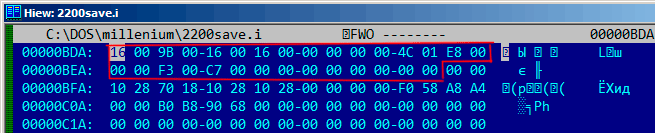
\includegraphics[scale=\FigScale]{ff/millenium/hiew3.png}
\caption{Hiew: \RU{первое состояние}\EN{state 1}}
\label{fig:mill_hiew3}
\end{figure}

\RU{Проверим каждое, и это они}\EN{Let's check each, and these are}.
\RU{Это явно 16-битные значения: не удивительно для 16-битной программы под DOS, где \Tint имел длину в 16 бит.}
\EN{These are clearly 16-bit values: not a strange thing for 16-bit DOS software where the \Tint type has 16-bit width.}

\clearpage
\RU{Проверим наши предположения}\EN{Let's check our assumptions}.
\RU{Запишем 1234 (0x4D2) на первой позиции (это должен быть водород)}%
\EN{We will write the 1234 (0x4D2) value at the first position (this must be hydrogen)}:

\begin{figure}[H]
\centering
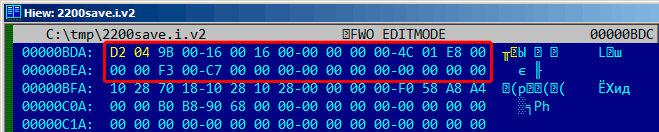
\includegraphics[scale=\FigScale]{ff/millenium/hiew4.png}
\caption{Hiew: \RU{запишем там}\EN{let's write 1234} (0x4D2)\EN{ there}}
\label{fig:mill_hiew4}
\end{figure}

\RU{Затем загрузим измененный файл в игру и посмотрим на статистику в шахте}%
\EN{Then we will load the changed file in the game and took a look at mine statistics}:

\begin{figure}[H]
\centering
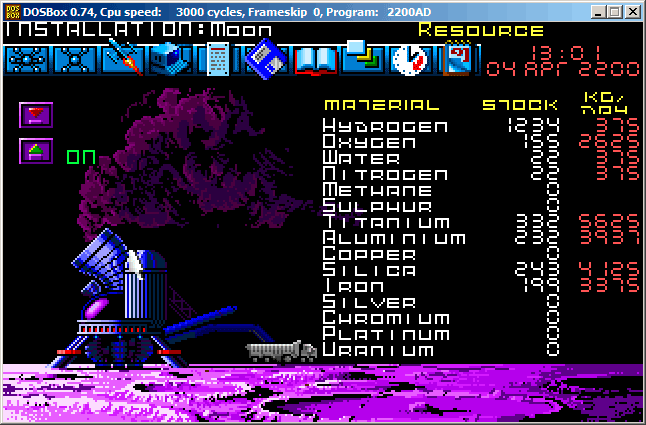
\includegraphics[scale=\FigScale]{ff/millenium/5.png}
\caption{\RU{Проверим значение водорода}\EN{Let's check for hydrogen value}}
\label{fig:mill_5}
\end{figure}

\RU{Так что да, это оно}\EN{So yes, this is it}.

\clearpage
\RU{Попробуем пройти игру как можно быстрее, установим максимальные значения везде}\EN{Now let's try to 
finish the game as soon as possible, set the maximal values everywhere}:

\begin{figure}[H]
\centering
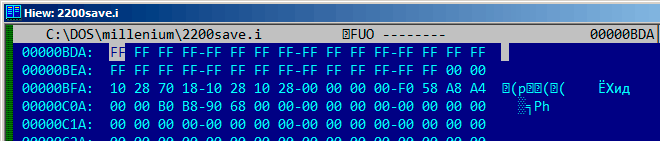
\includegraphics[scale=\FigScale]{ff/millenium/hiew7.png}
\caption{Hiew: \RU{установим максимальные значения}\EN{let's set maximal values}}
\label{fig:mill_hiew7}
\end{figure}

0xFFFF \RU{это}\EN{is} 65535, \RU{так что да, у нас много ресурсов теперь}\EN{so yes, we now have a 
lot of resources}:

\begin{figure}[H]
\centering
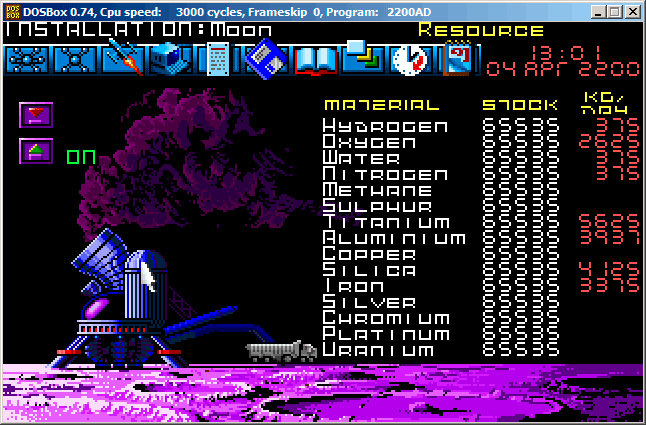
\includegraphics[scale=\FigScale]{ff/millenium/6.png}
\caption{\RU{Все ресурсы теперь действительно}\EN{All resources are} 65535 (0xFFFF)\EN{ indeed}}
\label{fig:mill_6}
\end{figure}

\clearpage
\RU{Пропустим еще несколько \q{дней} в игре и видим что-то неладное}\EN{Let's skip some \q{days} in the game and oops}! 
\RU{Некоторых ресурсов стало меньше}\EN{We have a lower amount of some resources}:

\begin{figure}[H]
\centering
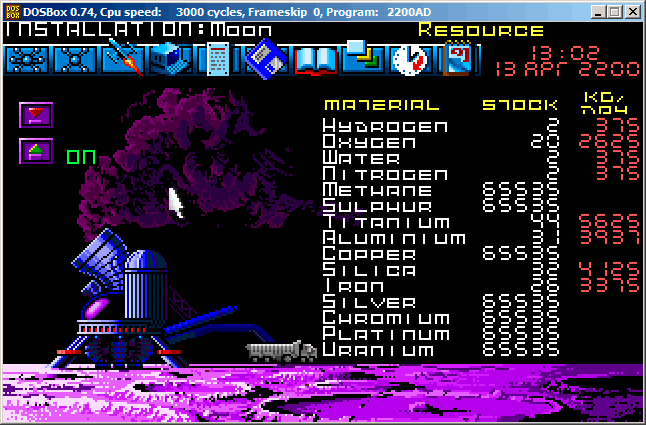
\includegraphics[scale=\FigScale]{ff/millenium/8.png}
\caption{\RU{Переполнение переменных ресурсов}\EN{Resource variables overflow}}
\label{fig:mill_8}
\end{figure}

\RU{Это просто переполнение}\EN{That's just overflow}. 
\RU{Разработчик игры вероятно никогда не думал, что значения ресурсов будут такими большими,
так что, здесь, наверное, нет проверок на переполнение, но шахта в игре \q{работает}, ресурсы добавляются,
отсюда и переполнение.}
\EN{The game's developer probably didn't think about such high amounts of resources,
so there are probably no overflow checks, but the mine is \q{working} in the game, resources are added,
hence the overflows.}
\RU{Вероятно, не нужно было жадничать}\EN{Apparently, it was a bad idea to be that greedy}.

\RU{Здесь наверняка еще какие-то значения в этом файле}\EN{There are probably a lot of more values 
saved in this file}.

\RU{Так что это очень простой способ читинга в играх}\EN{So this is very simple method of cheating in games}.
\RU{Файл с таблицей очков также можно легко модифицировать}\EN{High score files often can be easily 
patched like that}.

\EN{More about files and memory snapshots comparing}\RU{Еще насчет сравнения файлов и снимков памяти}: 
\myref{snapshots_comparing}.
